\documentclass[12pt]{article}
% General document formatting

\usepackage[utf8]{inputenc}
\usepackage[T1]{fontenc}
\usepackage{lmodern}

% Related to math
\usepackage{fullpage}
\usepackage{amsmath,amssymb,amsfonts,amsthm}
\usepackage{mathtools}
\usepackage{enumitem}

% Graphing
\usepackage[x11names]{xcolor}
\usepackage{tikz}
\usepackage{pgfplots}
\pgfplotsset{compat=newest}
\renewcommand{\thesubsection}{Question \arabic{subsection}}

\begin{document}
\begin{center}
{\Large\bf University of Waterloo}\\
\vspace{3mm}
{\Large\bf COURSE - TERM YEAR}\\
\vspace{2mm}
{\Large\bf Assignment #}\\
\vspace{3mm}
\textbf{Name: TJ Yang}\\
\textbf{Student Number:}
\end{center}

\section*{Part A}
\subsection{}
\begin{enumerate}[label=(\alph*)]
  \item
  \item
  \item
\end{enumerate}
\section*{Part B}
\begin{enumerate}
  \item
  \item
\end{enumerate}
\section*{Part C}

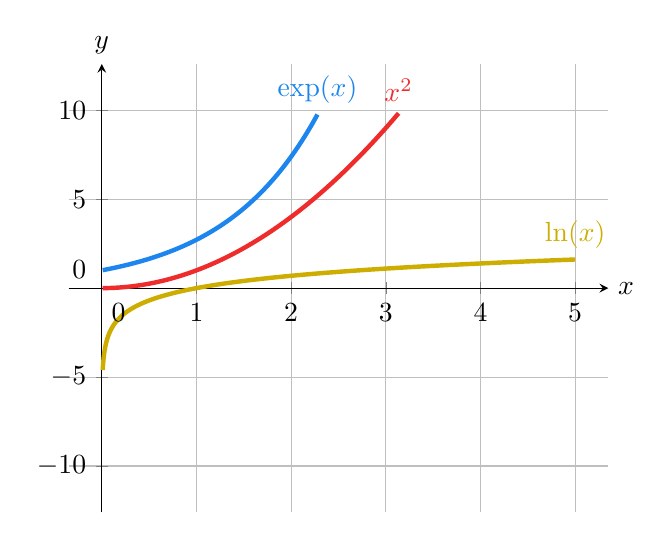
\begin{tikzpicture}
  \begin{axis}[
    grid = major,
    clip = true,
    clip mode=individual,
    restrict y to domain=-10:10,
    axis x line = middle,
    axis y line = middle,
    xlabel={$x$},
    xlabel style={at=(current axis.right of origin), anchor=west},
    ylabel={$y$},
    ylabel style={at=(current axis.above origin), anchor=south},
    domain = 0.01:5,
    xmin = 0,
    xmax = 5,
    enlarge y limits={rel=0.13},
    enlarge x limits={rel=0.07},
    ymin = -10,
    ymax = 10,
    after end axis/.code={\path (axis cs:0,0) node [anchor=north west,yshift=-0.075cm] {0} node [anchor=south east,xshift=-0.075cm] {0};},
  ]

    \addplot[color=Firebrick2,samples=100,smooth,ultra thick] {x^2} node[above,pos=1] {$x^2$};

    \addplot[color=DodgerBlue2,samples=100,smooth,ultra thick] {exp(x)} node[above,pos=1] {$\exp(x)$};

    \addplot[color=Gold3,samples=1000,smooth,ultra thick,unbounded coords=jump,no markers] {ln(x)} node[above,pos=1] {$\ln(x)$};

    %% Alternative %%

    % \addplot[color=Firebrick2,samples=100,smooth,ultra thick] {x^2} node[pos=1] (endofplotsquare) {};
    % \node [above,color=Firebrick2] at (endofplotsquare) {$x^2$};

    % \addplot[color=DodgerBlue2,samples=100,smooth,ultra thick] {exp(x)} node[pos=1] (endofplotsquare) {};
    % \node [above,color=DodgerBlue2] at (endofplotsquare) {$\exp(x)$};

    % \addplot[color=Gold3,samples=1000,smooth,ultra thick,unbounded coords=jump,no markers] {ln(x)} node[pos=1] (endofplotsquare) {};
    % \node [above,color=Gold3] at (endofplotsquare) {$\exp(x)$};
  \end{axis}
\end{tikzpicture}

\end{document}
